\documentclass[10pt,a4paper]{article}

\usepackage{fontspec}
\setmainfont{DMSans-Regular.ttf}[BoldFont=DMSans-Bold.ttf,ItalicFont=DMSans-Italic.ttf]
\setsansfont{DMSans-Regular.ttf}[BoldFont=DMSans-Bold.ttf,ItalicFont=DMSans-Italic.ttf]
\usepackage{microtype}
\usepackage[a4paper,top=1.7cm,bottom=1.7cm,left=1.6cm,right=1.6cm,headheight=22pt,headsep=8pt]{geometry}

\usepackage{amsmath,amssymb}
\usepackage{graphicx}
\graphicspath{{figures/}}
\usepackage{xcolor}
\usepackage{booktabs,array,tabularx,colortbl}
\usepackage{enumitem}
\usepackage{todonotes}
\usepackage{float}
\usepackage{needspace,etoolbox}
\pretocmd{\section}{\Needspace{5\baselineskip}}{}{}
\pretocmd{\subsection}{\Needspace{5\baselineskip}}{}{}
\usepackage{titlesec}
\usepackage{fancyhdr}
\usepackage{caption}
\usepackage{listings}
\usepackage[most]{tcolorbox}
\usepackage{tikz}
\usepackage[hidelinks]{hyperref}

\definecolor{navy}{HTML}{0A2233}
\definecolor{ink}{HTML}{173242}
\definecolor{gold}{HTML}{A59577}
\definecolor{paper}{HTML}{F7F5EF}
\definecolor{muted}{HTML}{59666B}
\definecolor{line}{HTML}{D9DCD7}
\hypersetup{colorlinks=true,linkcolor=navy,urlcolor=gold}

\color{ink}
\linespread{1.03}
\setlength{\parindent}{0pt}
\setlength{\parskip}{0.34em}

\newcommand{\tracked}[2][100]{{\addfontfeatures{LetterSpace=8}#2}}


\titleformat{\section}
  {\rmfamily\Large\color{navy}}
  {\textcolor{gold}{\thesection}\hspace{0.6em}}{0pt}{}
  [\vspace{-0.2em}{\color{gold}\titlerule[0.8pt]}]
\titleformat{\subsection}
  {\rmfamily\large\color{navy}}{\textcolor{gold}{\thesubsection}\hspace{0.5em}}{0pt}{}
\titleformat{\subsubsection}
  {\sffamily\bfseries\small\color{ink}\MakeUppercase}{}{0pt}{}
\titlespacing*{\section}{0pt}{2.2em}{1.2em}
\titlespacing*{\subsection}{0pt}{1.6em}{0.5em}
\titlespacing*{\subsubsection}{0pt}{.6em}{.15em}

\pagestyle{fancy}
\fancyhf{}
\renewcommand{\sectionmark}[1]{\markboth{#1}{}}
\fancyhead[L]{\small\textcolor{muted}{\tracked[120]{MERIDIAN CAPITAL}}}
\fancyhead[R]{\small\textcolor{muted}{\leftmark}}
\fancyfoot[L]{\footnotesize\textcolor{muted}{Asset Management Challenge 2026 \,$\cdot$\, Round 2}}
\fancyfoot[R]{\footnotesize\textcolor{navy}{\thepage}}
\renewcommand{\headrulewidth}{0.4pt}
\renewcommand{\footrulewidth}{0pt}
\renewcommand{\headrule}{\hbox to\headwidth{\color{gold}\leaders\hrule height \headrulewidth\hfill}}

\renewcommand{\arraystretch}{1.12}
\arrayrulecolor{line}
\newcommand{\hd}[1]{\textcolor{navy}{\textbf{#1}}}
\captionsetup{font={small,color=muted},labelfont={bf,color=navy},labelsep=period,skip=8pt}

\newtcolorbox{callout}[1][]{
  enhanced, breakable, colback=paper, colframe=paper,
  borderline west={2.5pt}{0pt}{gold},
  boxrule=0pt, arc=0pt, left=12pt, right=10pt, top=8pt, bottom=8pt,
  fonttitle=\bfseries\small, coltitle=navy, #1}

\lstdefinestyle{meridian}{
  language=Python, basicstyle=\ttfamily\footnotesize\color{ink},
  keywordstyle=\color{navy}\bfseries, commentstyle=\color{muted}\itshape,
  stringstyle=\color{gold}, numbers=left, numberstyle=\tiny\color{muted},
  numbersep=8pt, backgroundcolor=\color{paper}, frame=l, rulecolor=\color{gold},
  framesep=8pt, xleftmargin=14pt, breaklines=true, showstringspaces=false,
  columns=fullflexible, keepspaces=true}
\lstset{style=meridian}

\usepackage{tocloft}
\renewcommand{\cftsecfont}{\rmfamily\large\color{navy}}
\renewcommand{\cftsecpagefont}{\rmfamily\large\color{navy}}
\renewcommand{\cftsubsecfont}{\color{ink}}
\renewcommand{\cftsecleader}{\color{line}\cftdotfill{\cftdotsep}}
\setlength{\cftbeforesecskip}{0.9em}
\setcounter{tocdepth}{2}


\definecolor{editblue}{HTML}{D9EFFF}
\titlespacing*{\section}{0pt}{.8em}{.4em}
\titlespacing*{\subsection}{0pt}{.6em}{.2em}
\newcommand{\file}[1]{\texttt{\detokenize{#1}}}
\emergencystretch=3em

\begin{document}
\begin{titlepage}
\pagecolor{paper}
\thispagestyle{empty}
\color{navy}
\centering
\vspace*{0.6cm}

\makebox[\linewidth][c]{
\includegraphics[width=12.5cm]{Meridian-Capital-Official-Logo.png}}\par

\vspace{0.5cm}
{\color{gold}\rule{3.2cm}{0.8pt}\par}
\vspace{0.9cm}

{\rmfamily\fontsize{22}{28}\selectfont Tactical Deviation\par}
\vspace{0.4cm}
{\sffamily\color{muted}Discretionary Equity Investing: Valuation, Catalysts \& Performance\par}
\vspace{0.2cm}
{\sffamily\small\color{gold}\tracked[100]{ROUND 2 · ASSET MANAGEMENT CHALLENGE 2026 · REPORT}\par}

\vfill


\vspace{0.4cm}
{\sffamily\large\color{navy}
Alessia Battistella\\[3pt]
Tze Qing Ginnie Lee\\[3pt]
Katherine Lerner-Teves\\[3pt]
Kyla Kaplan\\[3pt]
Lorenzo Comi\par}

\vfill

{\color{gold}\rule{\textwidth}{0.4pt}\par}
\vspace{0.3cm}
{\sffamily\footnotesize\color{muted}
Universit\`a della Svizzera italiana \,$\cdot$\, Financial Modeling \,$\cdot$\, Prof.\ F.\ Franzoni\\[2pt]
November 2026\\[2pt]
}
\end{titlepage}
\nopagecolor
\color{ink}
\pagenumbering{roman}
\thispagestyle{plain}
\begingroup
\setlength{\parskip}{0pt}
\setcounter{tocdepth}{2}
\tableofcontents
\vfill
{\small Prices: 6 November 2026 close. Bloomberg entry: 7 November 2026.\\
The ten numbered pages that follow contain the report and complete portfolio description.}
\endgroup
\clearpage
\pagenumbering{arabic}

\section*{Introduction}
For Round 2, we add Adobe, Kroger, Hormel, Bristol Myers Squibb, Exxon and HP to the portfolio. We allocate one-third of the post-loss NAV to these six US-listed stocks and fund the purchases by reducing each ETF target to two-thirds of its original weight. The original six-ETF strategic asset allocation (SAA) remains our benchmark. At the 6 November close, NAV is \$97,115,068.58, including distributions. We choose the stock proportions using forecast alpha divided by residual variance. Monthly ex-ante tracking error is 3.92\%, within the challenge's required range, although the daily estimates show higher risk.

\section{Tactical Deviation}
\label{sec:deviation}

\subsection{Funding the Deviation}
We allocate one-third of NAV to stocks, following the instruction given in class. To fund this allocation, we reduce all six ETF targets proportionally. This keeps their relative weights unchanged and avoids making an additional call on which ETFs to sell more heavily. The original SAA is SPY 26.08\%, EEMV 9.66\%, DBC 26.95\%, SCHD 3.28\%, VGSH 5.00\% and STIP 29.03\%. The new ETF targets are 17.3867\%, 6.4400\%, 17.9667\%, 2.1867\%, 3.3333\% and 19.3533\%, respectively. Commodity exposure falls, but DBC remains a substantial position. Section~\ref{sec:implementation} gives the complete holdings and trade list.


\begin{center}

\begin{tikzpicture}[x=1cm,y=1cm,font=\sffamily\small]
\fill[gold!70] (0,0) rectangle (10.6,.55);
\fill[navy] (10.65,0) rectangle (15.9,.55);
\node[anchor=west,text=ink] at (.15,.28) {Two-thirds in the original ETFs};
\node[text=white] at (13.27,.28) {One-third in six stocks};
\end{tikzpicture}
\end{center}

\subsection{Tracking Error and Risk}
We estimate risk from 60 complete monthly USD total returns, covering November 2021--October 2026. We annualize the covariance matrix by multiplying it by 12 and calculate $TE=\sqrt{(w-w_B)'\Sigma(w-w_B)}$. Our annual TE falls within the required 2--5\% range. The tactical portfolio's estimated volatility is higher than the SAA's 8\% design target. For one-month 5\% VaR, we assume normally distributed returns with zero mean and use $1.645\,\sigma_{ann}/\sqrt{12}$. Losses can exceed this estimate.
\begin{center}\small
\begin{tabular}{lrr}\toprule
\hd{Metric} & \hd{SAA} & \hd{New portfolio} \\\midrule
Annual ex-ante tracking error & 0.00\% & 3.92\% \\
Annual ex-ante volatility & 7.89\% & 9.47\% \\
One-month 5\% VaR, loss / NAV & 3.74\% & 4.50\% \\\bottomrule
\end{tabular}\end{center}

\begin{center}
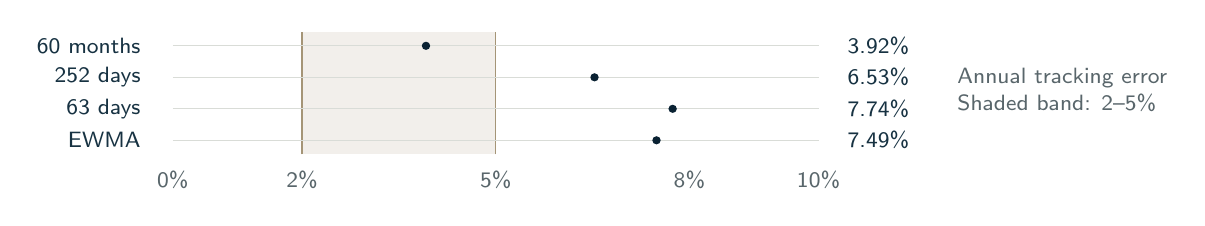
\begin{tikzpicture}[x=.82cm,y=.40cm,font=\sffamily\footnotesize]
\fill[gold!15] (2,-.45) rectangle (5,3.45);
\draw[gold] (2,-.45)--(2,3.45) (5,-.45)--(5,3.45);
\foreach \x in {0,2,5,8,10} {\node[anchor=north,text=muted] at (\x,-.65) {\x\%};}
\foreach \label/\val/\y in {60 months/3.92/3,252 days/6.53/2,63 days/7.74/1,EWMA/7.49/0} {
  \node[anchor=east,text=ink] at (-.35,\y) {\label};
  \draw[line,line width=.4pt] (0,\y)--(10,\y);
  \fill[navy] (\val,\y) circle[x radius=.065,y radius=.13];
  \node[anchor=west,text=ink] at (10.3,\y) {\val\%};
}
\node[anchor=west,align=left,text=muted] at (12,1.6) {Annual tracking error\\Shaded band: 2--5\%};
\end{tikzpicture}
\end{center}

\textbf{Additional checks.} Daily TE is 6.53\% over 252 sessions, 7.74\% over 63 sessions and 7.49\% with EWMA. These estimates exceed the 5\% level we use as an additional risk check, so the monthly result alone gives an incomplete picture. We also test the portfolio over 217 overlapping 33-session periods after DBC's methodology change on 10 November 2025. Average active return is $-0.395\%$, with outperformance in 44.2\% of periods. Each starting offset has only 6--7 non-overlapping windows, so these are far fewer than 217 independent tests. The block-bootstrap 95\% interval for mean active return is $[-1.30\%,+0.53\%]$. At ten historical forecast dates where monthly TE passed, realized 33-session TE subsequently exceeded 5\% in 80\% of cases. We test DBC's earlier methodology separately. The tests replay today's stock choices and assumptions across historical periods. Selection bias and the limited number of independent observations leave future outperformance uncertain.

\clearpage
\section{Stock Analysis and Valuation Dossier (Checkpoint 2)}
\label{sec:cp2}

We look for a valuation discount, a catalyst within the round and a reasonable contribution to risk relative to the SAA. We first value each company using normalized earnings and a P/E multiple, then check the result against cash flow, market-implied growth and returns under slower price adjustment. A low P/E is only useful if the earnings and cash flows behind it can be sustained. Entry prices are the 6 November USD close, and we assess catalyst timing against the round's 27 December end.


\subsection{ADBE -- Adobe Inc.}

\subsubsection*{Valuation}
We value Adobe at $18.145\times16=\$290.32$, using the midpoint of FY2026 GAAP EPS guidance and a 16x P/E. GAAP earnings include stock compensation. Our multiple is below the annual GAAP multiples of CRM, INTU and ORCL in the peer comparison, allowing for uncertainty over AI competition and renewals. We keep this comparison separate from adjusted analyst EPS. The FCFF valuation is \$271.14, still 13.3\% above the \$239.30 entry price. Adobe pays no dividend, which rules out a dividend-based valuation.

\subsubsection*{Value Trap Check}
Adobe's annual FCF margin and ROE are above both its earlier observations and the peer medians. Debt/equity and total payouts/FCF are less reassuring: both are worse than the historical and peer comparisons. Buybacks and leverage remain concerns despite strong subscription revenue. In the cash model, we charge SBC as an economic cost and avoid counting cash-flow adjustments twice. Annual FCF margin is 41.4\%, versus a prior-year mean of 38.1\% and a peer median of 34.7\%.

\subsubsection*{Specific Issues}
Cheaper AI tools and reverse-engineered product features could put pressure on prices and renewals. The effect of these tools on customer retention is still uncertain. We assess the risk through lower cash generation: a 10\% reduction in normalized cash gives a value of \$243.84, and a 20\% reduction gives \$216.54. Raising the required equity return by two percentage points gives \$224.90.

\subsubsection*{Catalyst}
Fiscal Q4 FY2026 results and the first FY2027 guidance, on 9 December 2026 after the US close, the first outlook under the new CEO. Adobe confirms the date in its investor calendar.\footnote{\href{https://www.adobe.com/investor-relations/calendar.html}{Adobe, investor calendar}.}

At \$239.30, Adobe trades about 17.6\% below our \$290.32 value, which implies only 13.2x FY2026 GAAP EPS. The market prices a structural threat from cheaper AI-native creative tools, and the FY2026 report is the first full-year test of that view. Execution so far has held up: in Q3 Adobe reported GAAP EPS of \$4.62 and non-GAAP EPS of \$6.13, on revenue of \$6.76B.

From 1 December, Anil Chakravarthy becomes CEO and Shantanu Narayen executive chair. The appointment is already public and adds no alpha, but the 9 December outlook will be the first test of the new team's priorities.

\textbf{What we will watch.}
\begin{itemize}[leftmargin=1.2em,itemsep=2pt,topsep=2pt]
  \item Recurring-revenue and renewal growth in line with or above the trend.
  \item Paid Firefly and AI Assistant features increasing total subscription revenue.
  \item FY2027 guidance consistent with continued earnings growth above our normalized \$18.15 GAAP EPS.
\end{itemize}

\textbf{Main risk.} A cut to FY2027 guidance, weaker renewals or signs of pricing pressure would confirm the market's disruption thesis and widen the discount.

\textbf{Timing and alpha.} One report is unlikely to close a 21\% gap in full. Applying the 50\% haircut in Section~\ref{sec:cp1} reduces the annual alpha estimate from 24.13\% to 12.07\%.

\subsection{KR -- The Kroger Co.}

\subsubsection*{Valuation}
We value Kroger at $5.20\times15=\$78.00$, compared with the \$67.70 entry price. EPS is the midpoint of FY2026 adjusted guidance. The 15x multiple is below the adjusted-forward peer median for ACI, WMT and TGT, although differences in their businesses limit the comparison. We use adjusted earnings because the e-commerce charges distort GAAP EPS. The FCFF valuation gives \$87.45. A dividend model would leave out retained cash and buybacks, which are important to Kroger's capital allocation.

\subsubsection*{Value Trap Check}
Kroger's annual ROE is below both its earlier mean and the peer median, while its FCF margin is stronger. Cash available without new borrowing covers dividends about 2.40 times. However, TTM buybacks of \$3.77bn exceed \$2.21bn of no-new-debt FCFE even before \$0.92bn of dividends. We therefore need to distinguish operating improvements from EPS growth supported by debt-funded buybacks. Annual FCF margin is 2.3\%, versus a prior-year mean of 1.4\% and a peer median of 2.1\%.

\subsubsection*{Specific Issues}
Thin grocery margins, wage costs and the fulfillment reset limit the multiple we are willing to pay. Interest-bearing debt is \$17.00bn. We exclude \$7.16bn of operating lease liabilities from financial debt because the lease payments are already included in operating cash flow. Deducting both would count the same obligation twice.

\subsubsection*{Catalyst}
Q3 FY2026 results on 3 December 2026. Analysts expect EPS of \$1.16, against \$1.05 in the same quarter a year ago.

At \$67.70 against a \$78.00 value (15x normalized adjusted EPS of \$5.20), Kroger trades at a discount to grocery peers. The discount reflects doubts about execution after the e-commerce reset: management recorded a \$2.6 billion impairment and related charges tied to its automated fulfillment network and closed three fulfillment centers. Q3 is the first full quarter to show whether the new model, with more fulfillment from stores, supports margins.

\textbf{What we will watch.}
\begin{itemize}[leftmargin=1.2em,itemsep=2pt,topsep=2pt]
  \item Identical sales growth excluding fuel, and a stable gross margin.
  \item FY2026 adjusted EPS guidance of \$5.10--5.30 reaffirmed or raised.
  \item Free cash flow that funds buybacks without more debt, since leverage is our main value-trap warning.
\end{itemize}

\textbf{Main risk.} A guidance cut, or EPS growth that comes only from buybacks while sales stall. Recent reactions show the stock moves on this report in both directions: +2.7\% in September and $-$8.4\% in June 2026.

\textbf{Timing and alpha.} The date is confirmed and the 15.2\% value/price gap offers room for a rerating. Kroger and Hormel both report on 3 December, so about 15\% of NAV reacts on the same day. Applying the 50\% haircut in Section~\ref{sec:cp1} reduces the annual alpha estimate from 16.29\% to 8.14\%.

\subsection{HRL -- Hormel Foods}

\subsubsection*{Valuation}
We value Hormel at $1.48\times17=\$25.16$, compared with the \$21.95 entry price. EPS is the midpoint of adjusted guidance of \$1.45--1.51; GAAP guidance is lower at \$1.06--1.12. Our 17x multiple assumes a recovery in margins and carries a premium to the adjusted-forward food peers TSN, SJM and CAG. That premium needs to be supported by results. FCFF gives \$31.49. The acquisition's funding needs also make future dividend forecasts uncertain.

\subsubsection*{Value Trap Check}
FCF margin, gross margin and payout coverage are weak against both Hormel's history and its peers. Its dividend record is encouraging, but current cash generation covers annual dividends only about 1.17 times. Adding acquisition debt reduces coverage to 1.10 times. With acquisition debt and full refinancing at our assumed rate, coverage falls to roughly 1.00. Annual FCF margin is 4.4\%, versus a prior-year mean of 7.3\% and a peer median of 8.7\%.

\subsubsection*{Specific Issues}
Brakebush costs \$1.055bn and requires new debt, while expected EPS accretion starts only in FY2028. We test dividend coverage under acquisition financing with operating benefits set to zero, a conservative assumption. The main business risks remain Retail volumes, input costs and integration.

\subsubsection*{Catalyst}
Fiscal Q4 FY2026 results and the first FY2027 outlook, on 3 December 2026 before the open. It is the first full outlook under the new CEO, John Ghingo, who took over from interim chief executive Jeff Ettinger on 26 October.\footnote{\href{https://www.just-food.com/?p=213435}{Just Food, Hormel to acquire Brakebush}.}

At \$21.95 against a \$25.16 value (17x FY2026 adjusted EPS of \$1.48), the market prices Hormel as a low-growth food company with structural margin problems. Recent results argue for a recovery: in Q3 Hormel raised its adjusted diluted EPS guidance to \$1.45--1.51, growth of 6\% to 10\%, and Foodservice recorded its 12th consecutive quarter of organic net sales growth.\footnote{\href{https://www.sec.gov/Archives/edgar/data/0000048465/000004846526000053/hormelearningsreleaseq32026.htm}{Hormel Foods, Q3 FY2026 earnings release (Form 8-K)}.} The same event moved the stock a year ago: the shares gained 3\% intraday after an in-line quarter and a more optimistic fiscal 2026 outlook.

\textbf{What we will watch.}
\begin{itemize}[leftmargin=1.2em,itemsep=2pt,topsep=2pt]
  \item FY2026 adjusted EPS delivered within the \$1.45--1.51 range.
  \item FY2027 guidance showing continued adjusted EPS growth, supporting the 17x multiple.
  \item Stable Retail volumes and margins, and cash flow that covers the dividend.
  \item A clear funding plan for Brakebush: the acquisition costs about \$1.055 billion, will be paid with cash on hand and new debt, and should add to adjusted EPS only from fiscal 2028.
\end{itemize}

\textbf{Main risk.} Weak FY2027 guidance, further Retail volume losses, or signs that the acquisition debt strains dividend coverage. Our valuation already carries a premium to food peers, so a disappointing outlook would remove its justification.

\textbf{Timing and alpha.} The date is confirmed and falls early enough for the price to adjust. Applying the 50\% haircut in Section~\ref{sec:cp1} reduces the annual alpha estimate from 15.58\% to 7.79\%.

\subsection{BMY -- Bristol Myers Squibb}

\subsubsection*{Valuation}
We value BMY at $6.45\times11=\$70.95$, compared with the \$62.14 entry price. EPS is the midpoint of FY2026 non-GAAP guidance of \$6.35--6.55. Our earnings input includes the disclosed IPRD/licensing cost. The 11x multiple allows for patent and pipeline risk relative to GILD, AMGN, MRK and ABBV. The flat-cash FCFF case gives a lower value of \$65.50. Patent losses make long-run dividend forecasts particularly uncertain.

\subsubsection*{Value Trap Check}
The comparisons of annual revenue growth, gross margin and leverage give us little reason to extrapolate current earnings indefinitely. We therefore assume zero cash growth in both valuation stages. A separate stress with a 2\% annual decline for five years gives \$58.59; a 10\% reduction in normalized cash gives \$57.48. Our flat-cash base case remains above the entry price, but the margin of safety is small. Annual FCF margin is 26.7\%, versus a prior-year mean of 27.6\% and a peer median of 25.6\%.

\subsubsection*{Specific Issues}
The pipeline must replace revenues lost as existing medicines lose exclusivity, while those medicines also fund new launches and debt service. We assess this risk through company-wide cash-flow scenarios. Valuing individual drugs would require separate estimates of trial success and commercial revenue. A failed or delayed readout could outweigh the apparent P/E discount.

\subsubsection*{Catalyst}
Two Phase III readouts expected by year-end, plus data at the ASH Annual Meeting on 12--15 December. Bristol Myers expects Phase III data for milvexian in secondary stroke prevention and for Sotyktu in lupus before year-end; the Q4 calendar also includes Cobenfy open-label Alzheimer's psychosis data at CTAD and Zenbexus progression-free survival data at ASH.\footnote{\href{https://finance.yahoo.com/quote/BMY/earnings/BMY-Q3-2026-earnings_call-660055.html}{BMY Q3 2026 earnings call transcript (Yahoo Finance)}.} The ASH meeting has fixed dates; the two Phase III readouts do not have a confirmed day.

At \$62.14 against a \$70.95 value (11x FY2026 non-GAAP EPS of \$6.45), BMY trades at only 9.6x guided earnings. The market discounts its patent cliff: Eliquis and Opdivo will lose exclusivity, and the pipeline has to replace them. Recent execution supports our value: after a strong third quarter BMY raised its 2026 guidance, with revenue up 7\% to about \$13.1 billion, growth-portfolio sales up 12\% and non-GAAP EPS guidance now \$6.35--6.55.\footnote{\href{https://www.marketbeat.com/earnings/reports/2026-10-29-bristol-myers-squibb-stock/}{MarketBeat, BMY Q3 2026 results}.} Management has reported four recent positive registrational readouts. Milvexian is the most important remaining program, as the potential successor to Eliquis.

\textbf{What we will watch.}
\begin{itemize}[leftmargin=1.2em,itemsep=2pt,topsep=2pt]
  \item Positive milvexian data in secondary stroke prevention, keeping the Eliquis-successor thesis alive ahead of the atrial-fibrillation study in 2027.
  \item Positive Sotyktu data in lupus, adding a large new indication to a growing product.
  \item Q4 sales confirming the raised guidance.
\end{itemize}

\textbf{Main risk.} A negative milvexian result would be the largest downside risk. The program already had a setback: BMY and Johnson \& Johnson stopped the Phase III Librexia ACS trial after an interim analysis found it unlikely to meet its primary efficacy endpoint. A further failure would deepen concerns about the patent cliff and our value-trap warnings: falling revenue, lower gross margin and rising leverage.

\textbf{Timing and alpha.} Two readouts are expected before year-end but have no fixed date, so either could fall after the 27 December cutoff; ASH gives one dated event inside the round. Applying the 50\% haircut in Section~\ref{sec:cp1} reduces the annual alpha estimate from 15.05\% to 7.52\%.

\subsection{XOM -- Exxon Mobil}

\subsubsection*{Valuation}
We value Exxon at $10\times18=\$180.00$, compared with the \$165.87 entry price. The \$10 EPS is our assumption for earnings across the commodity cycle. The 18x multiple requires sustained earnings from low-cost production, with CVX, COP and EOG as comparisons. We convert the same earnings assumption into cash using the 2023--25 median difference between CFO and net income. This gives an FCFF value of \$213.08, but the result still depends on the normalized earnings assumption.

\subsubsection*{Value Trap Check}
Exxon's annual ROE, FCF margin, gross margin and payout coverage are weaker than its historical and peer comparisons. Commodity prices remain the main influence on earnings and cash flow. Using lower-cycle historical CFO gives a value of about \$166.61, close to the entry price; increasing the required equity return by two percentage points gives \$139.08. We retain \$180 as the earnings-based value used to select the portfolio. Annual FCF margin is 7.3\%, versus a prior-year mean of 11.2\% and a peer median of 12.3\%.

\subsubsection*{Specific Issues}
To reach common equity value, we deduct annualized stock awards from cash generation and account for financial debt and minority interests. Operating lease payments remain in cash costs. We keep Exxon relatively small because the portfolio already has substantial commodity exposure through DBC. Dividend-only and book-value models would give too little weight to the commodity cycle and future investment needs.

\subsubsection*{Catalyst}
Start-up of the Uaru project offshore Guyana, and the 2027 corporate plan update expected later in Q4. Neither has a fixed date. Uaru is slated to begin oil production this year and will produce 250,000 barrels per day, taking Guyana's output to 1.15 million bpd; Exxon's Guyana president declined to give a specific start-up timeline.

At \$165.87 against a \$180.00 value (18x normalized EPS of \$10), the market discounts how durable Exxon's earnings are beyond the current oil price. A Uaru start-up on schedule and a 2027 plan showing production growth from low-cost barrels would support our normalized EPS, which sits below the FY2027 consensus but above the 2025 trough.

\textbf{What we will watch.}
\begin{itemize}[leftmargin=1.2em,itemsep=2pt,topsep=2pt]
  \item Uaru first oil announced before 27 December.
  \item 2027 guidance on capex, production and distributions supported by low-cost production under conservative oil-price assumptions.
\end{itemize}

\textbf{Main risk.} A fall in oil prices or refining margins, or a slip of Uaru or the plan update into 2027. The oil price can dominate any company-specific news, and Exxon adds energy exposure the portfolio already holds through DBC.

\textbf{Timing and alpha.} This is the weakest catalyst in the portfolio: no dated event, and a real risk that it falls after the cutoff. Applying the 50\% haircut in Section~\ref{sec:cp1} reduces the annual alpha estimate from 9.02\% to 4.51\%. The common 50\% assumption is generous for a catalyst without a firm date.

\subsection{HPQ -- HP Inc.}

\subsubsection*{Valuation}
We value HP at $2.38\times13.5=\$32.13$, compared with the \$28.46 entry price. Normalized GAAP EPS is the \$2.57 guidance midpoint less \$0.19 of tariff refunds. A separate adjusted-forward comparison with DELL, HPE and CSCO supports about \$32.98, although it uses a different EPS basis. FCFF gives \$34.44 after adjusting guided FCF for the refund proxy and SBC. Negative book equity makes P/B unsuitable.

\subsubsection*{Value Trap Check}
Negative equity also makes ROE and debt/equity difficult to interpret. We therefore focus on margins, cash coverage and financial debt. Our cash model starts from \$3.1bn of guided FCF, deducts a \$176m refund proxy and \$479m of SBC, then accounts for financing. This lets us assess payout capacity without assuming buybacks can continue indefinitely. Annual FCF margin is 5.1\%, versus a prior-year mean of 5.8\% and a peer median of 7.5\%.

\subsubsection*{Specific Issues}
Declining print demand, thin PC margins and higher memory costs could offset revenue growth. We remove the full-year tariff benefit of \$0.19 per share from recurring earnings, including the \$0.08 expected in Q4. A dividend model would also miss buybacks and rely heavily on management's choice of payout.

\subsubsection*{Catalyst}
Fiscal Q4 FY2026 results and FY2027 guidance, on 24 November 2026 after the close, confirmed by HP on 3 November.\footnote{\href{https://investor.hp.com/news-events/news/news-details/2026/HP-Inc--to-Announce-Fourth-Quarter-Fiscal-2026-Earnings-on-November-24-2026-and-to-Attend-Upcoming-Investor-Conferences/default.aspx}{HP, 3 November earnings-call announcement}.}

At \$28.46 against a \$32.13 value, the market doubts that HP can protect margins as memory costs rise and printing declines. The last two quarters argue the other way: Q3 FY2026 net revenue was \$15.7 billion, up 12.5\%, and HP raised its fiscal 2026 EPS and free cash flow outlook.\footnote{\href{https://www.earningswhispers.com/epsdetails/HPQ}{Earnings Whispers, HP Q3 FY2026 results}.} The FY2027 guidance is the event that can re-rate the stock, as a precedent shows: a year ago HP guided fiscal 2026 profit below expectations, and the shares fell 6\% in extended trading.\footnote{\href{https://ng.investing.com/news/earnings/hp-inc-shares-slide-after-softer-2026-earnings-forecast-2227859}{Investing.com, HP shares slide after softer 2026 forecast}.}

\textbf{What we will watch.}
\begin{itemize}[leftmargin=1.2em,itemsep=2pt,topsep=2pt]
  \item FY2027 EPS and free cash flow guidance that holds up after removing tariff refunds. The Q4 guidance includes an \$0.08 favorable impact from estimated tariff refunds; our \$2.38 normalized EPS already excludes them.
  \item PC pricing and mix offsetting higher memory costs.
  \item A steady rate of decline in print supplies.
\end{itemize}

\textbf{Main risk.} FY2027 guidance below normalized expectations or weaker cash generation. With negative book equity, the dividend and buybacks depend entirely on free cash flow.

\textbf{Timing and alpha.} The event is early in the round, leaving time for the price to adjust. Applying the 50\% haircut in Section~\ref{sec:cp1} reduces the annual alpha estimate from 14.45\% to 7.23\%.


\subsection{Cash-Flow and Reverse-Valuation Checks}
We discount five years of FCFF and a terminal perpetuity: $FCFF_0=CFO-\text{normalizations}-capex-SBC+\text{net interest}(1-t)$. CFO includes working capital, taxes and noncash adjustments. Investment income is removed before cash is added separately. WACC uses market equity less cash, financial debt (book-value proxy) and minority capital. CAPM uses the 4.84\% Treasury rate from 5 November, a 6.114\% ERP and the same 60-month market betas. Tax rates and borrowing spreads are our assumptions. We subtract debt and minority interests and add cash to reach common equity. The FCFE cross-check holds cash assumptions and market-value leverage consistent, retaining initial financing differences in cash. The FCFF and FCFE values agree when we apply the same financing assumptions. Both depend on our projected cash flows.
\begin{center}\small
\begin{tabular}{lrrrrrr}\toprule
\hd{Stock}&\hd{5y cash g}&\hd{Terminal g}&\hd{WACC}&\hd{FCFF value}&\hd{Lower value}&\hd{Implied g}\\\midrule
ADBE & 8.0\% & 3.0\% & 13.08\% & \$271.14 & \$271.14 & 4.89\% \\
KR & 3.0\% & 2.0\% & 6.31\% & \$87.45 & \$78.00 & 0.70\% \\
HRL & 2.0\% & 2.0\% & 6.20\% & \$31.49 & \$25.16 & -0.59\% \\
BMY & 0.0\% & 0.0\% & 5.83\% & \$65.50 & \$65.50 & -0.95\% \\
XOM & 2.0\% & 2.0\% & 5.83\% & \$213.08 & \$180.00 & 0.29\% \\
HPQ & 4.0\% & 3.0\% & 10.94\% & \$34.44 & \$32.13 & 1.57\% \\
\bottomrule\end{tabular}\end{center}
\begin{center}\footnotesize\setlength{\tabcolsep}{4pt}
\begin{tabular}{lrrrrrrrr}\toprule
\hd{Stock}&$FCFF_0$&\hd{Cash}&\hd{Debt}&\hd{Minority}&\hd{Shares}&\hd{Tax}&$r_D$&$k$\\\midrule
ADBE & 8,510.8 & 5,639.0 & 6,363.0 & 0.0 & 389.200 & 21\% & 5.34\% & 13.19\% \\
KR & 2,711.4 & 1,475.0 & 16,997.0 & 0.0 & 590.589 & 24\% & 5.84\% & 7.05\% \\
HRL & 795.3 & 868.4 & 2,855.1 & 0.0 & 550.351 & 24\% & 5.84\% & 6.52\% \\
BMY & 9,544.4 & 12,959.0 & 42,877.0 & 0.0 & 2,044.086 & 21\% & 5.84\% & 6.14\% \\
XOM & 33,690.3 & 12,153.0 & 34,250.0 & 6,731.0 & 4,079.222 & 21\% & 5.34\% & 5.89\% \\
HPQ & 2,663.9 & 4,169.0 & 9,160.0 & 0.0 & 901.791 & 21\% & 6.34\% & 12.06\% \\
\bottomrule\end{tabular}\end{center}
{\footnotesize Cash-flow and balance inputs are USD millions; shares are millions outstanding at 6 November. Flows are TTM except the stated XOM normalization and HPQ guidance; balances use the latest reported quarter. Tax and debt rates are assumptions. The workbook shows the CFO-to-FCFF bridge. Annual quality comparisons use the latest full fiscal year (2025, or January 2026 for KR), up to three earlier years, and the peer sets named above; growth has two earlier observations.}

As a conservative check, we take the lower of the earnings and FCFF values. We then solve for the cash growth that would justify the entry price, scaling cash flows to this lower valuation. The implied growth rates depend on the other model assumptions. We cannot identify duration when initial and terminal growth are equal, as in HRL, BMY and XOM. For KR and HPQ, there is no duration solution within 0--50 years. The large contribution from terminal value also makes the results sensitive to growth and discount rates.

We also calculate 1-, 3-, 5- and 10-year IRRs from dividends and the sale price. In one case the valuation gap closes at sale; in the other, the initial proportional discount persists. Dividends are paid out, remaining FCFE accumulates as cash at an after-tax Treasury yield, shares stay fixed and no future buybacks are assumed. The longer the gap takes to close, the smaller its contribution to annual returns. For Adobe, the cash-based annual IRR is 28.17\% if the gap closes after one year, 17.21\% if it closes after three years, and 12.43\% over three years if the discount persists. These scenarios illustrate returns over longer holding periods. We choose the 50\% alpha haircut in Section~\ref{sec:cp1} to allow for uncertainty over whether and when the valuation gap closes. The workbook and notebook contain the full cash schedules and growth/rate sensitivities.

\begin{center}
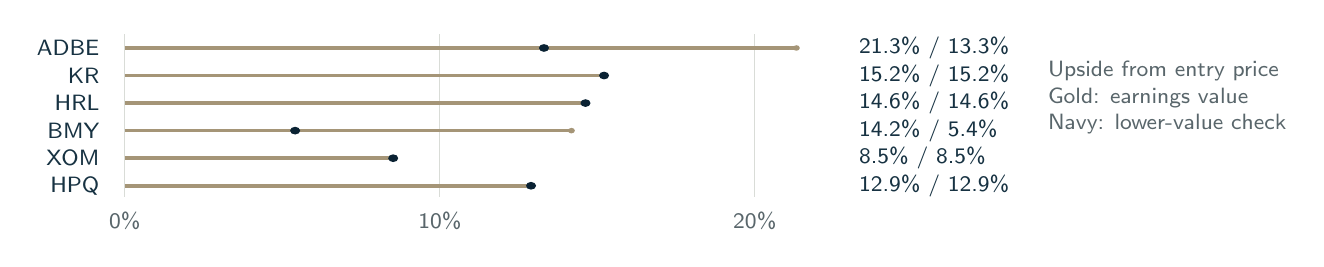
\begin{tikzpicture}[x=.40cm,y=.35cm,font=\sffamily\footnotesize]
\foreach \x in {0,10,20} {\draw[line] (\x,-.4)--(\x,5.5);\node[anchor=north,text=muted] at (\x,-.6) {\x\%};}
\node[anchor=east,text=ink] at (-.5,5) {ADBE};
\draw[gold,line width=1.3pt] (0,5)--(21.32052,5);
\fill[gold] (21.32052,5) circle[x radius=.11,y radius=.10];
\fill[navy] (13.30639,5) circle[x radius=.16,y radius=.14];
\node[anchor=west,text=ink] at (23,5) {21.3\% / 13.3\%};
\node[anchor=east,text=ink] at (-.5,4) {KR};
\draw[gold,line width=1.3pt] (0,4)--(15.21418,4);
\fill[gold] (15.21418,4) circle[x radius=.11,y radius=.10];
\fill[navy] (15.21418,4) circle[x radius=.16,y radius=.14];
\node[anchor=west,text=ink] at (23,4) {15.2\% / 15.2\%};
\node[anchor=east,text=ink] at (-.5,3) {HRL};
\draw[gold,line width=1.3pt] (0,3)--(14.62415,3);
\fill[gold] (14.62415,3) circle[x radius=.11,y radius=.10];
\fill[navy] (14.62415,3) circle[x radius=.16,y radius=.14];
\node[anchor=west,text=ink] at (23,3) {14.6\% / 14.6\%};
\node[anchor=east,text=ink] at (-.5,2) {BMY};
\draw[gold,line width=1.3pt] (0,2)--(14.17766,2);
\fill[gold] (14.17766,2) circle[x radius=.11,y radius=.10];
\fill[navy] (5.40441,2) circle[x radius=.16,y radius=.14];
\node[anchor=west,text=ink] at (23,2) {14.2\% / 5.4\%};
\node[anchor=east,text=ink] at (-.5,1) {XOM};
\draw[gold,line width=1.3pt] (0,1)--(8.51872,1);
\fill[gold] (8.51872,1) circle[x radius=.11,y radius=.10];
\fill[navy] (8.51872,1) circle[x radius=.16,y radius=.14];
\node[anchor=west,text=ink] at (23,1) {8.5\% / 8.5\%};
\node[anchor=east,text=ink] at (-.5,0) {HPQ};
\draw[gold,line width=1.3pt] (0,0)--(12.89529,0);
\fill[gold] (12.89529,0) circle[x radius=.11,y radius=.10];
\fill[navy] (12.89529,0) circle[x radius=.16,y radius=.14];
\node[anchor=west,text=ink] at (23,0) {12.9\% / 12.9\%};
\node[anchor=west,align=left,text=muted] at (29,3.2) {Upside from entry price\\Gold: earnings value\\Navy: lower-value check};
\end{tikzpicture}
\end{center}

\subsection{Rejected Candidates}
We researched nine positive-alpha stocks and compared all 420 combinations of three to six names. FDS, INTU and GILD were also considered, but we preferred the six-stock portfolio's balance of forecast IR, recent risk and concentration. The five-stock maximum has a full-residual IR of 0.698, compared with 0.696 for our six. However, its recent daily TE is 8.68\% and its largest stock weight is 9.09\%, compared with 7.74\% and 8.10\%. We accept the small reduction in forecast IR for those risk improvements. Our comparison is limited to the nine stocks we researched.

\section*{Data and Sources}
\begingroup\small
We use saved public prices, total returns and FRED Treasury rates. Entry prices are the 6 November close; risk estimates use November 2021--October 2026 monthly returns. The notebook records source dates, peer calculations, statement corrections and input hashes. Peer multiples use the earlier comparison snapshot, with annual GAAP and adjusted-forward EPS kept separate.

Our earnings assumptions use issuer releases: \href{https://www.sec.gov/Archives/edgar/data/796343/000079634326000147/adbeex991q326.htm}{Adobe Q3}; \href{https://ir.kroger.com/news/news-details/2026/Kroger-Reports-Second-Quarter-2026-Results-and-Updates-Guidance-for-2026/default.aspx}{Kroger Q2}; \href{https://www.hormelfoods.com/wp-content/uploads/Hormel-Earnings-Release-Q3-2026_FINAL.pdf}{Hormel Q3}; \href{https://www.bms.com/assets/bms/us/en-us/pdf/investor-info/doc_financials/quarterly_reports/2026/BMY-Q3-2026-Earnings-Press-Release-0039.pdf}{BMY Q3}; \href{https://investor.exxonmobil.com/company-information/press-releases/detail/1213/exxonmobil-announces-third-quarter-2026-results}{Exxon Q3}; and \href{https://www.hp.com/content/dam/sites/garage-press/press/press-releases/2026/q3-fy26-earnings/HP_Inc_Reports_Q3FY26_Earnings.pdf}{HP Q3}. Catalyst dates are checked against issuer calendars. We have no confirmed date for an Exxon investor day or the BMY readouts. The \href{https://github.com/kybeka/meridian-capital/tree/main/research/round-2}{Round 2 repository} contains the reproducible notebooks and Excel model, which use the same NAV and share quantities as this report.
\endgroup
\clearpage
\section{Alphas and Portfolio Weights}
\label{sec:cp1}
\textit{Class 3, Part II. We estimate alphas and weights from the earnings-based valuations, with cash-flow values used as a sensitivity.}

For each stock, $k_i=r_f+\beta_{i,M}ERP$. If the price reaches our value after one year, the full-convergence scenario gives $\alpha_i^{full}=(1+k_i)(V_i/P_i-1)$. We use half of this estimate: $\alpha_i=0.5\alpha_i^{full}$, applying the same 50\% haircut to all six stocks. Residuals come from regressing monthly excess stock returns on SAA excess returns, $r_i-r_f=a_i+\beta_{i,B}(r_B-r_f)+\varepsilon_i$. We annualize their sample variance by 12. Valuations provide our forecast alphas, and the regressions provide betas and residual risk. We use the valuation premia as SAA-relative alpha inputs. The market-based discount rate gives a required return for each stock; outperformance against the SAA depends on the benchmark's return as well. Prices are from 6 November, and the risk estimates use 60 complete months ending October 2026.

\begin{center}\small\setlength{\tabcolsep}{5pt}
\begin{tabular}{lrrrrrrr}\toprule
\hd{Stock}&\hd{Price}&\hd{Value}&\hd{MoS}&\hd{Base alpha}&$\beta_{i,B}$&$\sigma_\varepsilon$&\hd{Fund weight}\\\midrule
ADBE & 239.30 & 290.32 & 17.57\% & 12.07\% & 2.086 & 34.81\% & 4.65\% \\
KR & 67.70 & 78.00 & 13.21\% & 8.14\% & 1.255 & 21.66\% & 8.10\% \\
HRL & 21.95 & 25.16 & 12.76\% & 7.79\% & 0.521 & 22.96\% & 6.90\% \\
BMY & 62.14 & 70.95 & 12.42\% & 7.52\% & 0.989 & 23.55\% & 6.33\% \\
XOM & 165.87 & 180.00 & 7.85\% & 4.51\% & 1.681 & 24.12\% & 3.62\% \\
HPQ & 28.46 & 32.13 & 11.42\% & 7.23\% & 2.122 & 30.08\% & 3.73\% \\
\bottomrule\end{tabular}\end{center}
MoS is $1-P/V$, while the upside used to calculate alpha is $V/P-1$. Prices and values are in USD per share.

\subsubsection*{Why the alphas are positive}
\textbf{ADBE:} earnings and cash generation support a value above entry; the 9 December outlook will test renewals and paid AI demand. \textbf{KR:} normalized grocery earnings and the 3 December margin update support the case. \textbf{HRL:} the 3 December outlook must show recovery while preserving dividend coverage. \textbf{BMY:} pipeline readouts could reduce concern over the patent cliff. \textbf{XOM:} Uaru and corporate-plan news could support normalized earnings, although timing is uncertain. \textbf{HPQ:} the confirmed 24 November outlook will test earnings after tariff refunds. Several events fall after the next 28--29 November rebalance, so their timing needs to be considered separately from the annual alpha estimates.

\subsubsection*{Weights}
Following the long-only weighting rule, $b_i=\max(\alpha_i,0)/\sigma_{\varepsilon i}^{2}$, $x_i=b_i/\sum_j b_j$, and each stock's fund weight is $w_i=x_i/3$. Stocks with negative alpha receive zero weight. The six scores are 0.996, 1.735, 1.477, 1.357, 0.776 and 0.799. Kroger receives the largest weight because its relatively low residual risk produces a high alpha/variance score. Its 8.10\% weight is slightly above our additional 8\% preference. We retain the calculated weight because applying a cap would change the required proportions.

The stock basket's annual forecast alpha is 8.002\%, with an SAA beta of 1.312 and full-covariance residual volatility of 11.499\%. Its contribution to fund alpha is 2.667\% of NAV per year. The classroom formula, which omits residual correlations, gives $IR=\sqrt{\sum_i\alpha_i^2/\sigma_{\varepsilon i}^2}=0.756$. Including those correlations gives $IR_A=\alpha_A/\sqrt{x'\Omega x}=0.696$. Both estimates measure forecast alpha per unit of residual risk. The fund's active TE also captures the effect of its different SAA beta, giving a broader measure of active risk.

\subsubsection*{Fundamental Law and credibility}
The Fundamental Law provides a useful check on these forecasts. For six independent decisions and an illustrative $IC=0.10$, $IR=IC\sqrt{6}=0.245$. Our diagonal estimate instead implies $IC=0.756/\sqrt{6}=0.309$, which would require much stronger forecasting skill. Correlations reduce effective diversification, and the challenge's short horizon limits the number of independent investment decisions. Likewise, $S_P^2=S_B^2+IR_A^2$ describes the theoretical Sharpe benefit under optimal beta-adjusted mixing and valid alphas; its applicability is limited by our fixed one-third stock allocation and uncertainty over the alphas. Under the illustrative Fundamental Law estimate, the theoretical gain is $\sqrt{S_B^2+0.245^2}-S_B$, conditional on those assumptions.

Holding the weights fixed, the conservative cash-flow values reduce forecast residual IR to 0.564. Reducing all original fair values by 5\% lowers it to 0.426. We therefore treat 0.696 as an optimistic estimate. Valuations and catalysts support our stock choices. The historical tests and daily risk estimates leave considerable uncertainty about outperformance during the round.
\clearpage
\section{Performance of the First Round}
\label{sec:performance}
\subsection{Return, Volatility and Sharpe Ratio}
From 16 October to 6 November, our Round 1 portfolio fell from \$100m to \$97,115,068.58, a return of $-2.885\%$. We calculate daily NAV from the opening quantities and public closing prices, recognizing distributions on the ex-date and avoiding a second count when they are paid. Across 15 daily returns, annualized realized volatility is 8.14\%, slightly above the 8\% target, and annualized Sharpe is $-6.50$. We calculate Sharpe as $\sqrt{252}\,\overline{(r_p-r_f)}/s(r_p-r_f)$ using the daily Treasury proxy. With so few observations, this annualized ratio is highly sensitive to the losses during the period.

\subsection{Performance Attribution}
\begin{center}\small
\begin{tabular}{lrrrr}\toprule
\hd{Position}&\hd{Opening weight}&\hd{Holding return}&\hd{P\&L, USD}&\hd{Contribution, pp}\\\midrule
SPY & 26.08\% & -3.66\% & -955,365.24 & -0.955 \\
EEMV & 9.66\% & -3.58\% & -346,049.90 & -0.346 \\
DBC & 26.95\% & -6.52\% & -1,757,263.20 & -1.757 \\
SCHD & 3.28\% & 2.39\% & 78,300.16 & +0.078 \\
VGSH & 5.00\% & 0.62\% & 31,106.22 & +0.031 \\
STIP & 29.03\% & 0.22\% & 64,340.53 & +0.064 \\
\midrule Total & 100.00\% & & $-2,884,931.42$ & $-2.885$\\\bottomrule
\end{tabular}\end{center}
\begin{center}
\begin{minipage}[t]{.48\linewidth}\centering
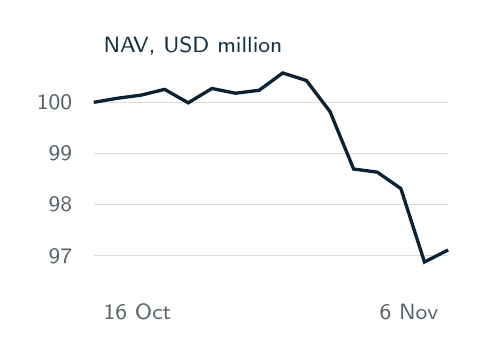
\begin{tikzpicture}[x=.30cm,y=.65cm,font=\sffamily\footnotesize]
\node[anchor=west,text=ink] at (0,5.1) {NAV, USD million};
\foreach \y/\label in {1/97,2/98,3/99,4/100} {\draw[line] (0,\y)--(15,\y);\node[anchor=east,text=muted] at (-.5,\y) {\label};}
\draw[navy,line width=1.2pt] plot coordinates {(0,4.000000) (1,4.079079) (2,4.140011) (3,4.252669) (4,3.989779) (5,4.269962) (6,4.177341) (7,4.234939) (8,4.573123) (9,4.426399) (10,3.818845) (11,2.696845) (12,2.635169) (13,2.314541) (14,0.879595) (15,1.115069)};
\node[anchor=north west,text=muted] at (0,.25) {16 Oct};\node[anchor=north east,text=muted] at (15,.25) {6 Nov};
\end{tikzpicture}\end{minipage}\hfill\begin{minipage}[t]{.48\linewidth}\centering
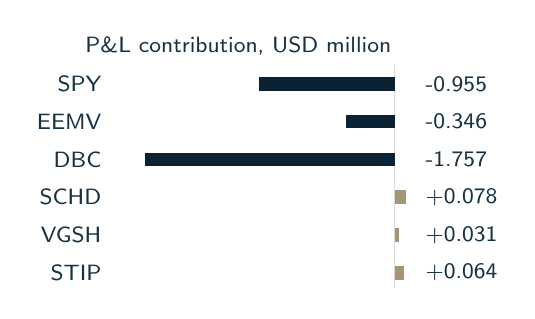
\begin{tikzpicture}[x=1.8cm,y=.48cm,font=\sffamily\footnotesize]
\node[anchor=west,text=ink] at (-2.25,6) {P\&L contribution, USD million};
\draw[line] (0,-.4)--(0,5.5);
\node[anchor=east,text=ink] at (-2,5) {SPY};
\fill[navy] (0,4.82) rectangle (-0.955365,5.18);
\node[anchor=west,text=ink] at (.15,5) {-0.955};
\node[anchor=east,text=ink] at (-2,4) {EEMV};
\fill[navy] (0,3.82) rectangle (-0.346050,4.18);
\node[anchor=west,text=ink] at (.15,4) {-0.346};
\node[anchor=east,text=ink] at (-2,3) {DBC};
\fill[navy] (0,2.82) rectangle (-1.757263,3.18);
\node[anchor=west,text=ink] at (.15,3) {-1.757};
\node[anchor=east,text=ink] at (-2,2) {SCHD};
\fill[gold] (0,1.82) rectangle (0.078300,2.18);
\node[anchor=west,text=ink] at (.15,2) {+0.078};
\node[anchor=east,text=ink] at (-2,1) {VGSH};
\fill[gold] (0,0.8200000000000001) rectangle (0.031106,1.18);
\node[anchor=west,text=ink] at (.15,1) {+0.031};
\node[anchor=east,text=ink] at (-2,0) {STIP};
\fill[gold] (0,-0.18) rectangle (0.064341,0.18);
\node[anchor=west,text=ink] at (.15,0) {+0.064};
\end{tikzpicture}\end{minipage}
\end{center}

We calculate each contribution as the holding's P\&L, including entitled dividends, divided by initial \$100m NAV. DBC contributed $-1.757$ percentage points, accounting for about 61\% of the net loss. SPY contributed a further $-0.955$ points, while SCHD, VGSH and STIP partly offset the losses. This experience supports reducing commodity exposure in Round 2. Even after the reduction, DBC and Exxon leave the portfolio exposed to energy prices.

Closing NAV includes \$12.12 of opening cash and the distributions paid before 6 November: \$16,372.15 from VGSH (86,671 shares $\times\$0.1889$, ex 2 November, paid 4 November) and \$84,544.63 from STIP (288,630 $\times\$0.292917$, ex 2 November, paid 5 November). Securities alone were worth \$97,014,139.67. Our website initially showed \$97,014,152.14 because it omitted these distributions and differed by \$0.35 in its securities prices. We corrected it to include both payments.

\clearpage
\section{Portfolio Description}
\label{sec:implementation}
\subsection{Portfolio implementation}
We entered the rebalance in Bloomberg on \textbf{7 November 2026}, using \textbf{6 November 2026 closing prices}. All positions are in \textbf{USD}. With NAV of \$97,115,068.58, the one-third stock budget is \$32,371,689.53. We calculate $q_i^*=w_iC/P_i$ and convert this to whole shares, with no fees or reserve. The final entries include one additional SPY share and one additional Adobe share to reduce unused cash.

\begin{center}\footnotesize\setlength{\tabcolsep}{4pt}
\begin{tabularx}{\linewidth}{@{}X l r r r@{}}\toprule
\hd{Security}&\hd{Bloomberg ID}&\hd{Shares}&\hd{Weight \%}&\hd{Trade shares}\\\midrule
SPDR S\&P 500 ETF & SPY US & 22,964 & 17.39 & -11,205 \\
iShares EM Min Vol ETF & EEMV US & 89,717 & 6.44 & -43,893 \\
Invesco DB Commodity ETF & DBC US & 553,213 & 17.97 & -245,543 \\
Schwab US Dividend ETF & SCHD US & 60,380 & 2.19 & -35,108 \\
Vanguard Short-Term Treasury ETF & VGSH US & 55,948 & 3.33 & -30,723 \\
iShares 0--5 Year TIPS ETF & STIP US & 186,996 & 19.35 & -101,634 \\
Adobe Inc. & ADBE US & 18,865 & 4.65 & +18,865 \\
The Kroger Co. & KR US & 116,215 & 8.10 & +116,215 \\
Hormel Foods Corp. & HRL US & 305,167 & 6.90 & +305,167 \\
Bristol Myers Squibb & BMY US & 99,004 & 6.33 & +99,004 \\
ExxonMobil Holdings Corp. & XOM US & 21,201 & 3.62 & +21,201 \\
HP Inc. & HPQ US & 127,276 & 3.73 & +127,276 \\
\midrule Cash & USD & & 0.00 & \\
\hd{Total} & & & \hd{100.00} & \\\bottomrule
\end{tabularx}\end{center}
All Bloomberg identifiers use the Equity market sector, for example SPY US Equity. Positive trade quantities are purchases and negative quantities are sales; every trade uses the 7 November entry date and 6 November 2026 price date. We retain full precision in the calculations and round weights only for display. Securities total \$97,114,952.53 and remaining cash is \$116.05. The stocks total \$32,371,559.04, or 33.33320\% of NAV. Whole-share rounding explains the \$130.49 difference from the exact one-third budget.

Closing prices (USD): SPY 735.29; EEMV 69.71; DBC 31.54; SCHD 35.17; VGSH 57.86; STIP 100.51; ADBE 239.30; KR 67.70; HRL 21.95; BMY 62.14; XOM 165.87; HPQ 28.46.

Full descriptions of all twelve securities and their sources accompany the portfolio description.
\end{document}
